\newpage
\chapter{Решение задачи Дирихле с разрывными граничными условиями на прямоугольнике}

\section{Постановка задачи}
\begin{equation}
	\begin{cases}
		\Delta u = 0, \\
		u(0, y) = 0,&u(a, y)=0,\\
		u(x, 0) = 0,&u(x, b)=f(x),
	\end{cases}
\end{equation}
где $f(x) = \alpha I_{[l,r]}(x)$.

\section{Аналитическое решение}
Воспользуемся методом разделения переменных. Будем искать решение в виде
\begin{equation*}
	u(x,y) = X(x)Y(y).
\end{equation*}
Получаем систему уравнений
\begin{equation}
	\frac{X''(x)}{X(x)}=-\frac{Y''(y)}{Y(y)}=-\lambda.
\end{equation}
Задача Штурма-Лиувилля для $X(x)$:
\begin{equation}\label{sl1}
	\begin{cases}
		X''(x)+\lambda X(x)=0,\\
		X(0)=X(a)=0.
	\end{cases}
\end{equation}

Получаем собственные значения:
\begin{equation*}
	\sqrt{\lambda_n}=\mu_n=\frac{\pi n}{a} .
\end{equation*}
Собственные функции для задачи (\ref{sl1}) с точностью до константы имеют вид
\begin{equation*}
	X_n(x)=\sin{\mu_n x}.
\end{equation*}
Задача для $Y(y)$:
\begin{equation}\label{sl2}
	\begin{cases}
		Y_n''(x)-\lambda_n Y_n(x)=0,\\
		Y_n(0)=0.
	\end{cases}
\end{equation}
Имеем
\begin{equation}
	Y_n(y)=C_{n_1}e^{-\mu_n  y}+C_{n_2}e^{\mu_n  y}
\end{equation}
\begin{equation*}
	Y_n(0)=C_{n_1} + C_{n_2} = 0.
\end{equation*}
Значит,
\begin{equation}
	Y_n(y)=C_n \sh{\mu_n y}
\end{equation}
\begin{equation}
	u(x,y) = \sum_{n=1}^{\infty}C_n \sh{\mu_n y} \sin{\mu_n x}
\end{equation}
\begin{equation*}
	C_n = \frac{2}{b sh{\mu_n b}}\int_0^b f(x) \sin{\mu_n x} \dd{x} = \frac{2\alpha}{b\sh{\mu_n b}}\int_l^r\sin{\mu_nx}\dd{x} =  \frac{2\alpha}{b\mu_n\sh{\mu_n b}}(\cos{\mu_n l} - \cos{\mu_n r})=
\end{equation*}
\begin{equation}
	=\frac{4\alpha}{b\mu_n\sh{\mu_n b}}\sin{\frac{\mu_n}{2}(l+r)}\sin{\frac{\mu_n}{2}(r-l)}.
\end{equation}
Окончательное решение:
\begin{equation}
	u(x,y)=\frac{4\alpha}{b}\sum_{n=1}^{\infty}\frac{\sin{\left(\frac{\mu_n}{2}(l+r)\right)}\sin{\left(\frac{\mu_n}{2}(r-l)\right)}}{\mu_n\sh{\mu_n b}}\sh{\mu_n y} \sin{\mu_n x}.
\end{equation}

\section{Вариационная формулировка задачи}
Домножим уравнение $\Delta u = 0$ на тестовую функцию $v$ и проинтегрируем по области $\Omega = (0,a)\times(0,b)$:
\begin{equation}
	\int_{\Omega}v \Delta u \dd{\Omega}=0.
\end{equation}
По формуле интегрирования по частям,
\begin{equation}
	\int_{\Omega}v \Delta u \dd{\Omega}=\int_{\partial \Omega}v\frac{\partial u}{\partial n}\dd{S}-\int_{\Omega}\nabla v\nabla u \dd{\Omega}=-\int_{\Omega}\nabla v \nabla u \dd{\Omega}.
\end{equation}
Слабая формулировка задачи:
\begin{equation}\label{weak_form}
	\int_{\Omega} \nabla v \nabla u \dd{\Omega}=0
\end{equation}

\section{Визуализация}
Визуализация для случая $a=b=1$, $n=30$, $\alpha = 0.05$.
%\begin{center}
\begin{figure}[t]
	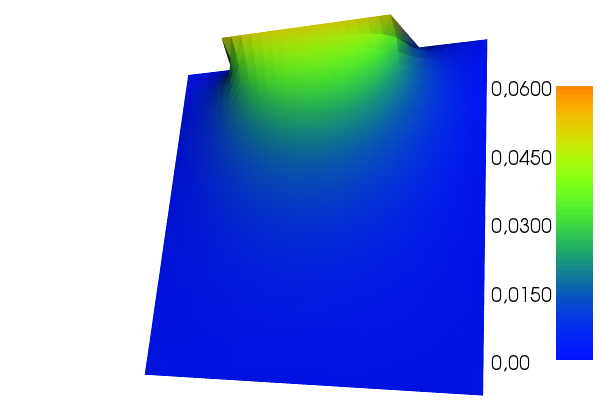
\includegraphics[scale=0.4]{dolfin_plot_0.png}
	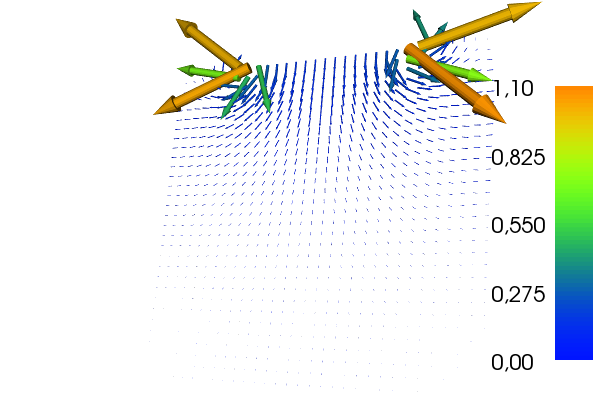
\includegraphics[scale=0.4]{dolfin_plot_1.png}
	\caption{Визуализация потенциала и напряжённости, полученных методом конечных элементов}
	\centering
	%\end{center}
\end{figure}

\section{Оценка скорости сходимости численного решения}
Зададим шаг равномерной прямоугольной сетки $h=\frac{1}{n}$. Произведём эксперименты с $h_0>h_1>h_2>...$ и получим соответствующие невязки $e_0, e_1, e_2, ...$. Предположим, что $e_i=Ch_i^r$. По результатам 2-ух экспериментов можно оценить $r$:
\begin{equation}
	r = \frac{\ln{\frac{e_{i+1}}{e_i}}}{\ln{\frac{h_{i+1}}{h_i}}}.
\end{equation}

Далее приведены результаты серии вычислений. Для вычисления погрешности использовалась $L_2$-норма.
\center{
\begin{tabular}{|l|l|l|}
	\caption{погрешность метода в серии вычислений}
    \hline
    n&e&r\\
    \hline
    8& 0.00164702& 1.999999999999731\\
	16& 0.00041175& 1.999999999999871\\
	32& 0.00010294& 1.999999999999943\\
	64& 0.00002573& 1.999999999999973\\
	128& 0.00000643& 1.99999999999982\\
	256& 0.00000161& 1.999999999999992\\
	\hline
\end{tabular}
}
